%% ============================================================================
\section{Introduction}
\label{sec:intro}

AI coding agents are increasingly deployed in production software development environments, yet evaluating these agents reliably remains challenging.
Organizations must frequently compare foundation models, validate changes to agent configurations, and assess infrastructure updates, decisions that require fast, reproducible evaluation signals.
However, the available evaluation methods involve trade-offs.

Online evaluation through A/B testing yields high-fidelity signals grounded in real interactions, but requires weeks to achieve statistical significance, consumes substantial engineering resources, and risks degrading user experience during experimentation.
Shadow deployment runs candidate agents in parallel with production systems without serving their outputs to users, avoiding user disruption. However, it introduces non-determinism, as model outputs and environment state vary across runs, undermining reproducibility.

Offline evaluation using existing benchmarks offers speed and reproducibility, but public benchmarks differ from production workloads in multiple ways.
SWE-Bench~\cite{jimenezSWEbenchCanLanguage2024}, for example, sources tasks from Python GitHub issues, which differ from industrial workloads in programming language distribution (predominantly Python versus polyglot codebases), prompt style (structured issue descriptions versus informal developer requests), and codebase structure (standalone repositories versus large-scale monorepos).

These observations motivate a benchmark derived directly from production data that:
(1) preserves verbatim prompts rather than reconstructing them synthetically;
(2) reflects the actual distribution of programming languages and task types in the target deployment; and
(3) provides stable, execution-based evaluation signals suitable for both rapid experimentation and reinforcement learning.

This paper presents \benchmark{}, a benchmark curated from real sessions with a production AI coding assistant.
Each sample consists of a verbatim prompt, the corresponding committed code change (hereafter referred to as a \emph{diff}, following industry convention for a patch or pull request), and a set of fail-to-pass (F2P) tests, tests that fail before the change and pass after, providing an automated correctness signal without requiring LLM-based judges.
The benchmark spans seven programming languages, reflecting the language distribution of a large industrial codebase.
To help ensure reliability, the curation pipeline applies multiple filtering stages: LLM-based task classification to identify testable coding tasks, test relevance validation to confirm tests exercise the changed code, and multi-run stability checks to exclude flaky tests.

Evaluation across four foundation models shows solve rates ranging from \SolveRateLowest{}\% to \SolveRateHighest{}\%, with \SolveRateBestModel{} achieving the highest performance.
Analysis of tool usage patterns reveals that models making greater use of work validation tools, such as running tests and checking for errors, achieve higher solve rates, suggesting that iterative verification improves agent effectiveness on proprietary codebases.

This paper makes the following contributions:
\begin{itemize}
\item A replicable methodology for constructing AI coding agent benchmarks from production sessions, providing verbatim prompts and execution-based evaluation across multiple programming languages in a monorepo setting.
\item A data curation pipeline that addresses monorepo-specific challenges, including environment reproducibility, test selection, and flaky test mitigation, to produce reliable evaluation signals.
\item A systematic analysis of model and harness evaluations run on this benchmark with implications for harness engineering and model deployment.
\end{itemize}

The benchmark dataset is not publicly released. However, the methodology, filtering criteria, and lessons learned described in this paper are replicable: organizations with access to their own production data can follow the same approach to construct analogous benchmarks tailored to their environments.

%% ============================================================================
\section{Benchmark Goals and Challenges}
\label{sec:challenges}

\benchmark{} is designed around three goals: (1) reflect realistic developer prompts, (2) operate in a large industrial monorepo, and (3) provide a reliable execution-based evaluation signal, each of which introduces specific challenges.

\paragraph{Realistic prompts.}
We aim to evaluate agents on prompts that match how developers actually use coding assistants.
Prompts reconstructed from diff metadata or templated task descriptions can be convenient, but they may be systematically different from real requests (e.g., missing context, overly formal, or biased toward what is easy to label).
A robust benchmark with a verified link between the natural-language conversation in which a developer issued a request and the corresponding code commit that fulfilled it helps ensure that each prompt--task pair faithfully represents real developer intent.

\paragraph{Should work in a monorepo (the ``time travel'' problem).}
Building a benchmark from a large-scale monorepo introduces infrastructure constraints that do not appear in small open-source repositories.
Unlike settings where one can check out an old commit and deterministically re-run historical tooling and tests, industrial monorepos use distributed services and ephemeral artifacts that make ``time travel'' difficult.
Developer tooling such as code search, semantic indexing, and file navigation often runs as remote services that continuously index the latest codebase state and provide only limited historical lookback, causing drift when evaluating older revisions.
Similarly, command-line tools and compiler binaries are deployed through package managers with automatic expiration (e.g., 30--365 days), preventing long-term use of archived toolchains.
Build systems and type checkers frequently use precomputed repository-wide indices that expire within days to weeks, and regenerating them on older commits may fail due to incompatibilities with current tooling.
Finally, contextual signals such as CI logs and failure traces are typically retained only briefly, and strict deployment policies may prohibit executing outdated code against production-adjacent services.
Together, these constraints motivate a rolling benchmark design where samples are periodically refreshed rather than frozen indefinitely.

\paragraph{Reliable evaluation signal.}
A benchmark is only useful if it yields a trustworthy pass/fail signal.
First, many real requests are not directly testable via execution (e.g., documentation-only changes, code explanation, UI-only tweaks), so the curation pipeline must filter to tasks that can be meaningfully evaluated with automated tests.
Second, even for testable tasks, naively running the entire continuous integration (CI) suite per candidate is often computationally expensive in a monorepo.
One practical solution is test discovery and relevance filtering: selecting a small set of tests that are actually affected by the change and that produce stable fail-to-pass behavior, rather than relying on coincidental failures, flakiness, or unrelated regressions.




%% ============================================================================
\section{\benchmark{}}
\label{sec:curation}

\benchmark{} is an execution-based benchmark for evaluating AI coding agents. The tasks are curated from real sessions with a production coding assistant. Figure~\ref{fig:funnel} illustrates the data funnel, showing how the initial pool of conversations is progressively filtered to yield high-quality benchmark samples.

\begin{figure*}[t]
\centering
\begin{minipage}[b]{0.48\textwidth}
\centering
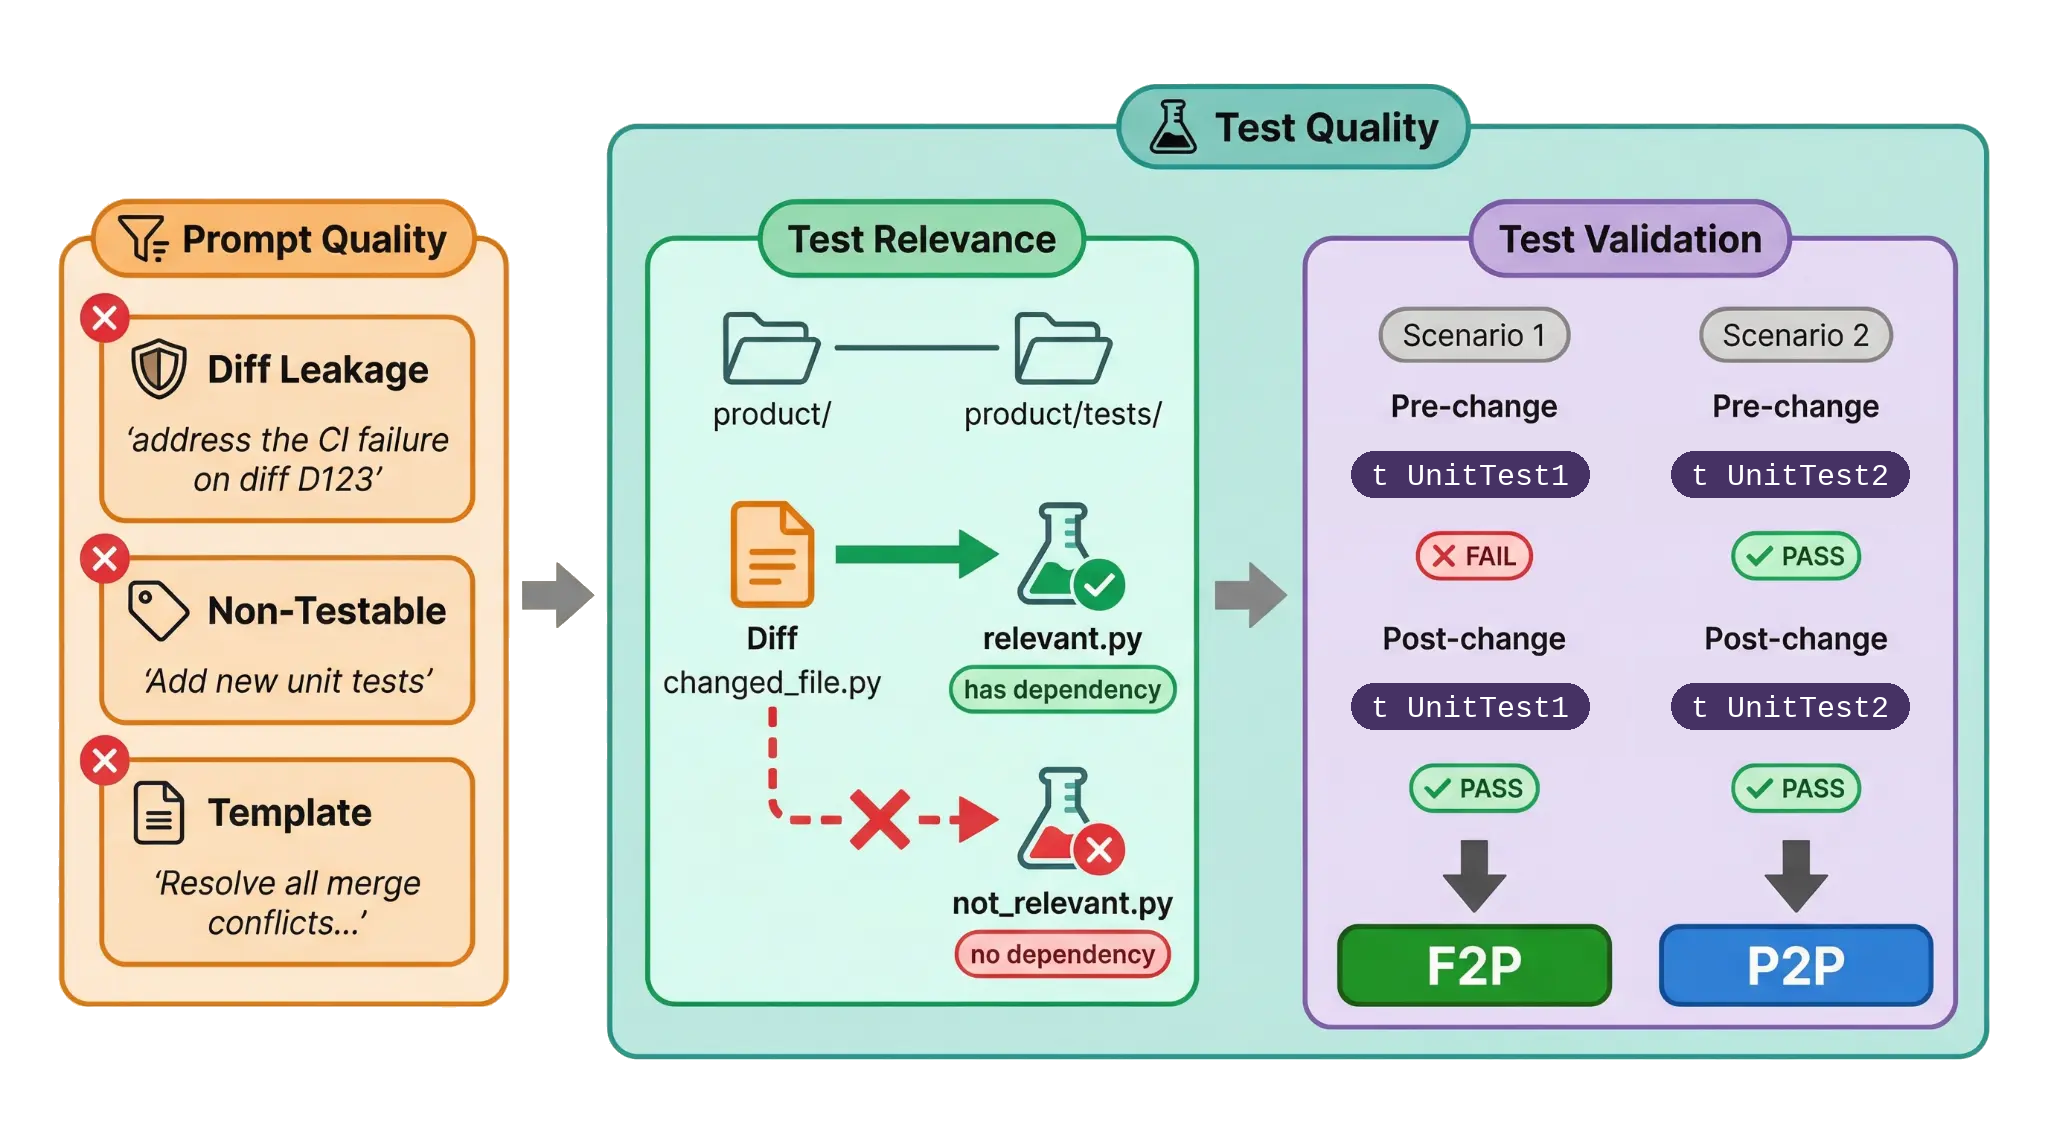
\includegraphics[width=\textwidth]{images/verification_v2_nobg.png}
\end{minipage}
\hfill
\begin{minipage}[b]{0.48\textwidth}
\centering
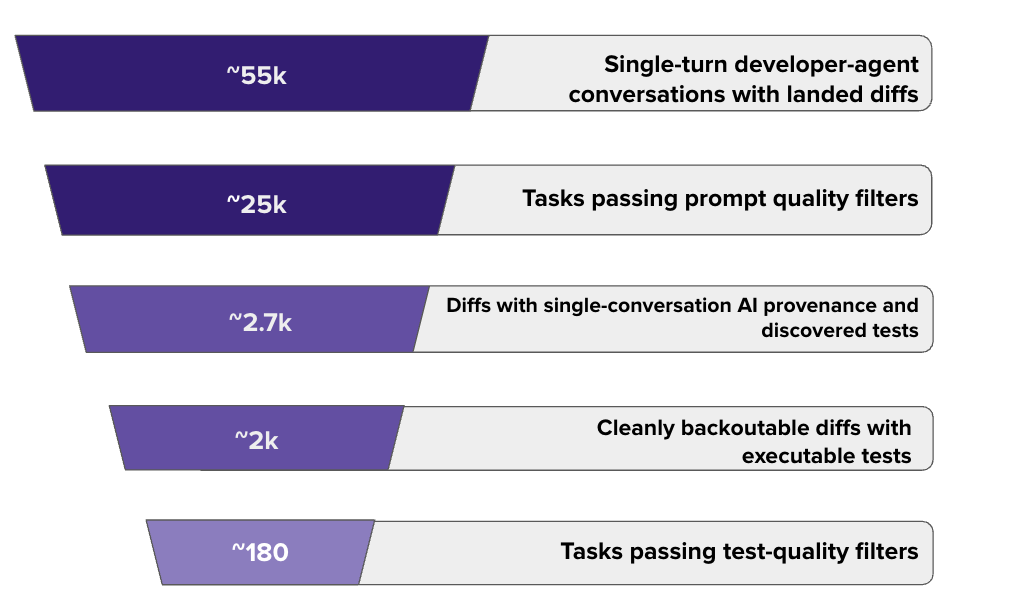
\includegraphics[width=\textwidth]{images/funnel_diagram.png}
\end{minipage}
\caption{\normalfont \benchmark{} verification pipeline. (Left) Starting from real developer-agent conversations, we apply prompt quality filters and test quality filters to obtain high-quality benchmark tasks with reliable fail-to-pass evaluation signals. (Right) Data funnel showing how the initial pool of conversations is progressively filtered to yield high-quality benchmark samples.}
\label{fig:funnel}
\end{figure*}

\subsection{Task Representation}
\label{subsec:task}

Each benchmark task consists of three components: prompt, a solution diff, and a set of executable tests. The prompt is a natural language request from a real session, preserving the actual phrasing and context used when interacting with the coding assistant. The solution diff represents the code changes that were subsequently approved, merged, and committed (i.e., \emph{landed}) to the main branch in response to the prompt. The tests provide an execution-based evaluation signal for the agent's code changes.

\benchmark{} tasks are interactive and the agent is expected to use the tools at its disposal to navigate the monorepo and produce a patch in response to the prompt. The solution diff is hidden from the agent at evaluation time and the executable tests run at the end of the agent trajectory to verify the expected outcome. We do not employ any LLM judges~\cite{zhengJudgingLLMasajudgeMTbench2023}, relying exclusively on the executable tests to provide an evaluation signal. The tasks in the benchmark are harness-agnostic and support evaluations for both internal and external agents, including Claude Code.

\subsection{Dataset Construction}
\label{subsec:construction}

We construct the dataset from ground-up using raw developer-agent trajectories which resulted in a committed diff in the repository.

\paragraph{Realistic Tasks}

We source data from authentic conversations between developers and an AI coding assistant integrated into an IDE. We filter on single-turn conversations where a developer provides a single natural language prompt and the agent produces code changes without intermediate human feedback.
We focus on single-turn sessions for two reasons: (1) multi-turn sessions require simulating human responses during evaluation, introducing additional complexity and synthetic prompts, and (2) enough sessions are single-turn to provide sufficient volume.

Each single-turn conversation is mapped to a solution diff that was subsequently approved, merged, and committed to the monorepo. The IDE is instrumented to record every keystroke and to log whenever AI-generated content, whether from code completion or conversational coding agents, is accepted by the developer and retained in the final committed diff. This \emph{AI provenance} metric enables us to track the connection between a conversation and its resulting landed diff, and to quantify the proportion of each diff that originates from AI suggestions. To maintain a strict one-to-one mapping between developer intent and code modifications, we exclude diffs that resulted from more than one developer-agent conversation. This helps ensure that the developer's request is not underspecified at the time of evaluation, enabling reliable evaluation of whether an agent's output matches the expected solution.

\paragraph{Evaluation Integrity}

As discussed in Section~\ref{sec:challenges}, monorepo infrastructure constraints can prevent reproducing the exact environment at a past commit. However, hiding the solution diff from the agent's environment helps ensure the agent does not ``cheat'' on a task by reading the committed solution files. We achieve this by backing out the solution diff from the current repository and running the agent evaluation on top of the backed out commit. Due to the dynamic nature of a large codebase, some diffs cannot be cleanly backed out due to conflicting changes and are excluded from the benchmark.

\paragraph{Evaluation Signal}

We employ probabilistic test retrieval to discover tests associated with each diff. We ensure only healthy, reliable tests are returned.
We explicitly exclude flaky, failing, or disabled tests from the discovery phase. The test discovery step also ensures that retrieved tests are executable on the latest version of the master branch.

\paragraph{Rolling Benchmark}

\benchmark{} is designed as a \emph{rolling benchmark}, one that periodically refreshes its task set with recent samples rather than remaining fixed, to keep benchmark volume healthy despite filters on conversation length and test availability. This design also helps ensure the benchmark stays fresh, contamination-free, and in-distribution with current development practices.


\subsection{Verification}
\label{subsec:verification}

To obtain a reliable evaluation signal from the dataset, we apply a series of rigorous filters to obtain a high-quality benchmark.

\vspace{1em}
\textbf{Prompt Quality Filters}


\paragraph{Solution Diff Leakage}
We identified cases where prompts referenced the ``solution diff,'' the diff created as a result of the conversation. While solution diffs are hidden from the agent at evaluation time by backing out the change from the repository, an agent can still access a previous diff, if explicitly asked to. For example, prompts like ``address the CI failure on diff D123'' can lead the agents to query the version control system and retrieve the solution compromising evaluation integrity. To prevent agents from exploiting this reference, we remove any conversations that reference the solution diff in the developer's request.

\paragraph{Non-Testable Prompts.} We use an LLM-powered classifier to filter prompts based on whether they can be reliably evaluated with automated tests. We exclude tasks where test verification is infeasible (e.g., test generation, documentation-only changes, UI-only modifications) and retain testable tasks such as bug fixes, feature requests, and refactoring.

\paragraph{Template Prompts}
We exclude conversations where the developer message matches known system prompts or template messages. These automated messages do not represent genuine developer-agent interactive coding tasks. Common patterns include conversation summarization requests, automated diff creation prompts, and merge conflict resolution templates.


\vspace{1em}
\textbf{Test-Quality Filters}
\paragraph{Test Relevance Filtering.} An agentic classifier validates that for each (diff, test) pair, the test is affected by the code changes, either directly or indirectly through dependencies. To evaluate candidate tests for a diff, we build a Test Relevance Agent and equip it with a diff content fetching tool and a code search subagent. The agent's purpose is to review the code and file changes and understand if a test can be impacted by the code changes. Previously, test discovery picked up transient test failures as relevant fail-to-pass tests that demonstrated inconsistent behavior at evaluation time due to test flakiness. This step improves upon the probabilistic test discovery by improving the precision of the candidate tests for the diff, subsequently improving eval reliability.


\paragraph{Test Validation and Classification.} The Test Relevance Agent does not execute tests so it does not distinguish between fail-to-pass and pass-to-pass behavior for tests. In order to classify tests, we execute the remaining tests on both the pre-change and post-change versions. We run each test multiple times to ensure reliability and exclude any spurious failures due to caching or setup problems. This final validation step produces the test classification into F2P (Fail-to-Pass) and P2P (Pass-to-Pass) which forms the basis for the benchmark's evaluation signal. Inconsistent tests are excluded from those categories and are stored separately. A no-op validation is run with the final benchmark that runs an agent evaluation with no code edits and expectedly yields a 0.0\% solve rate.

%% ============================================================================
\subsection{Benchmark Composition}
\label{sec:benchmark}

\label{subsec:distribution}

The benchmark includes a diverse mix of task types, with bug fixes, feature requests, and refactoring being the most common categories. Figure~\ref{fig:task-categories} shows the distribution of tasks in \benchmark{}.

\paragraph{Language Distribution} The benchmark spans multiple programming languages reflecting the real-world diversity of developer workflows and ensures the benchmark evaluates agents across different language ecosystems.

\paragraph{Test Distribution} \benchmark{} has two test categories based on their behavior. \textit{Fail-to-Pass (F2P)} tests fail or are broken on the pre-change version but pass on the post-change version, these serve as the primary evaluation signal. \textit{Pass-to-Pass (P2P)} tests pass on both versions and serve as regression tests to ensure changes do not break existing functionality. Tests with unreliable execution are excluded from the final benchmark. Note that ``Fail-to-Pass'' characterizes the test behavior, not necessarily bug-fixing; F2P tests may exercise new functionality, API extensions, or other behavioral changes, not only defect repairs. Approximately 75\% of tasks in the benchmark have at least one F2P test, while the remaining 25\% rely solely on P2P tests for evaluation.

\paragraph{Prompt Realism.}
One contribution of \benchmark{} is capturing \textit{authentic} developer-agent interactions rather than synthetic task descriptions.
A qualitative review of the collected prompts surfaced several emergent themes that set \benchmark{} apart from synthetic task descriptions.
Compared to synthetic benchmarks, these prompts more often (i) assume enterprise context and implicit knowledge, such as internal vocabulary and domain-specific shorthand tied to internal tooling conventions; (ii) center on debugging from real breakage, where developers ask agents to investigate regressions introduced by prior changes and to perform root-cause analysis before proposing a fix; and (iii) require pattern following, asking the agent to propagate changes by identifying an existing example and applying it consistently throughout the codebase.

\begin{figure}[t]
\centering
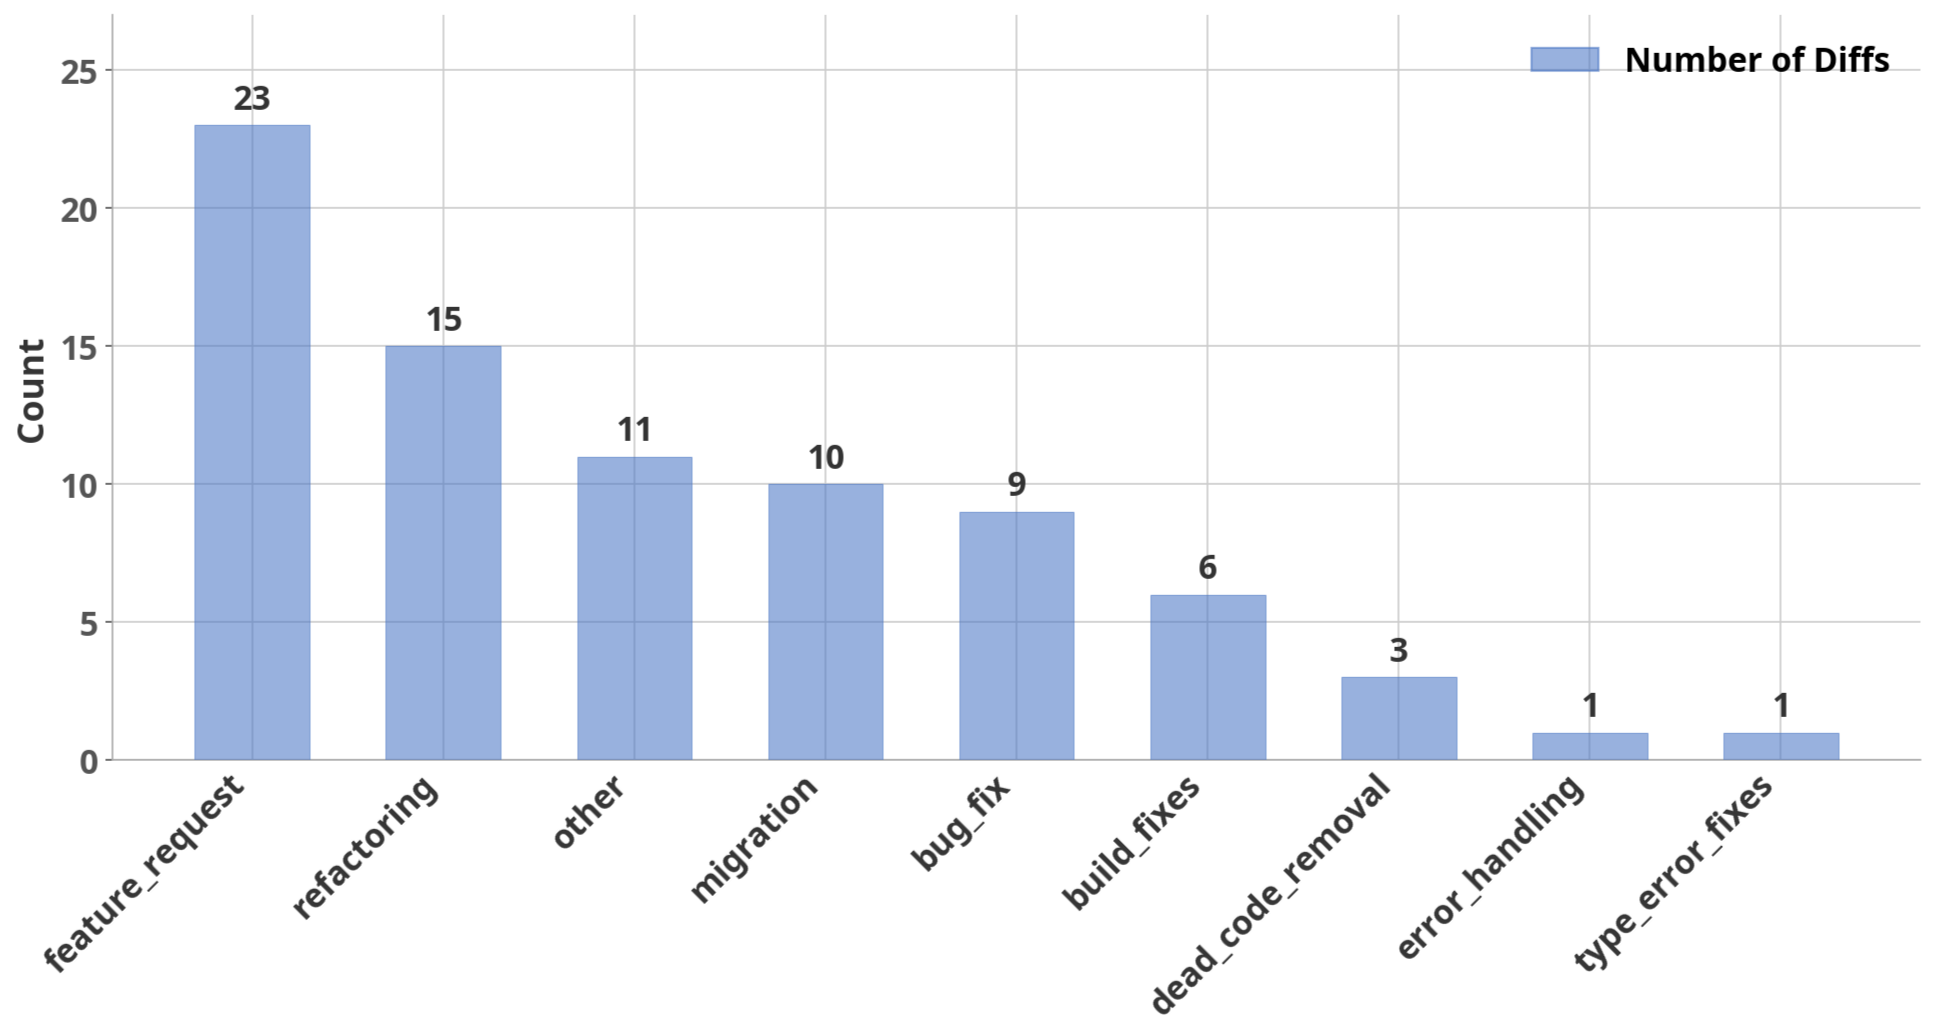
\includegraphics[width=0.9\columnwidth]{images/benchmark_task_level_vertical.png}
\caption{\normalfont Tasks per category in \benchmark{}, assigned by an LLM-powered task classifier based on prompt content.}
\label{fig:task-categories}
\end{figure}

%% ============================================================================
\section{Evaluation Results}
\label{sec:evaluation}

\begin{figure*}[t]
\centering
\begin{minipage}[b]{0.48\textwidth}
\centering
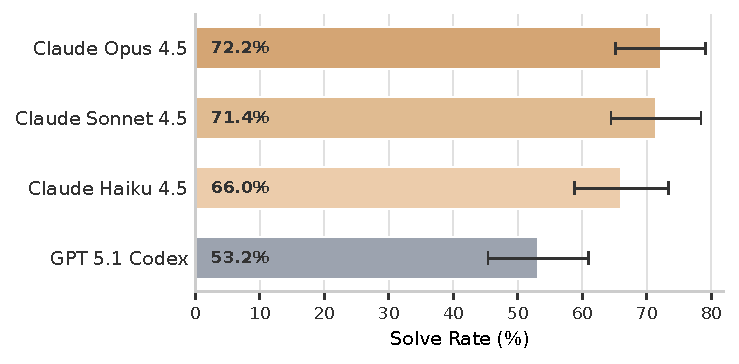
\includegraphics[width=0.9\textwidth,height=0.25\textheight,keepaspectratio]{images/dm_bench_multi_model_comparison.pdf}
\end{minipage}
\hfill
\begin{minipage}[b]{0.48\textwidth}
\centering
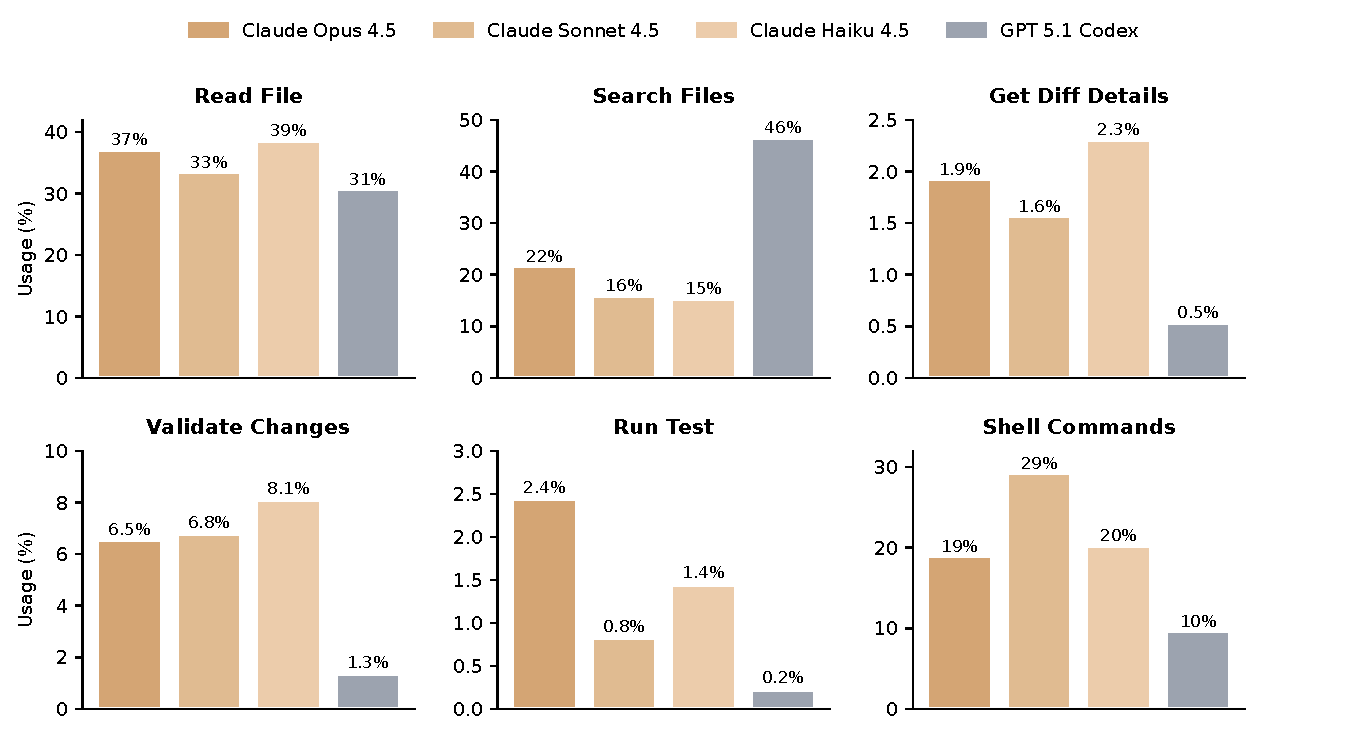
\includegraphics[width=1.0\textwidth]{images/dm_bench_tool_insights.pdf}
\end{minipage}
\caption{\normalfont Frontier model evaluations on \benchmark{}. (Left) Model solve rates with 95\% confidence intervals. (Right) Tool usage distribution across the same models demonstrating that Claude models have higher validation and testing rates compared to GPT Codex. All models are running on the same harness.}
\label{fig:model-eval}
\end{figure*}

We present evaluation results across three dimensions: model performance comparison, harness evaluation, and qualitative analysis. We run the evaluation on the F2P subset of the benchmark, i.e., only on diffs that have at least one fail-to-pass test.
\subsection{Model Evaluation}
We evaluated multiple large language models on \benchmark{} using the fail-to-pass subset of the benchmark. Each model was evaluated three times to measure variance. Figure~\ref{fig:model-eval} (left) presents the solve rates with 95\% confidence intervals.
The evaluation results reveal clear performance tiers among the models. Claude Opus achieves the highest solve rate, followed by Claude Sonnet. This suggests that models from the same family scale predictably with capability.

\begin{insight}
Unlike open-source benchmarks where models may have seen the codebase during training, internal monorepos are entirely unknown to the model. Static analysis and runtime verification can become important for models to verify their work. Industry practitioners should ensure coding agents have access to validation mechanisms to unleash their full potential on proprietary codebases.
\end{insight}

\subsection{Harness Evaluation}
We compare two evaluation harnesses on \benchmark{}. \textbf{Agent-Basic} uses a more limited toolset and simpler search tools. \textbf{Agent-IDE} features a comprehensive toolset with prompts designed to generalize across both GPT and Claude series models. The Agent-IDE harness has roughly 3x more tools than Agent-Basic, reflecting a full IDE-like experience: code navigation, local diagnostics, formatting, and knowledge search. Additionally, we evaluate the effect of \textbf{Context Files}, which are developer-authored Markdown files that encode internal codebase knowledge such as coding conventions, build system details, and project-specific patterns. These files can be loaded at evaluation time to help the agent navigate the proprietary codebase.

Figure~\ref{fig:harness-eval} presents the results. Model variance is observed on the weaker Agent-Basic harness, where Opus 4.6\footnote{The harness comparison uses Opus 4.6, which became available after the main leaderboard evaluation was conducted with the Claude 4.5 model family.} significantly outperforms GPT 5.1 Codex but individual models perform similarly with the stronger Agent-IDE harness. The addition of Context Files lifts the solve rate on Agent-Basic harness. We observed that coding languages with heavy company-specific conventions benefit the most from centralized context files. Conversely, more standardized languages gain less from company-specific context files.

\begin{insight}
A stronger, IDE-like harness boosts solve rates vs.\ a weaker barebone harness. With strong tooling, model gaps shrink. Context Files help most when harnesses are weak.
\end{insight}

\begin{figure}[t]
\centering
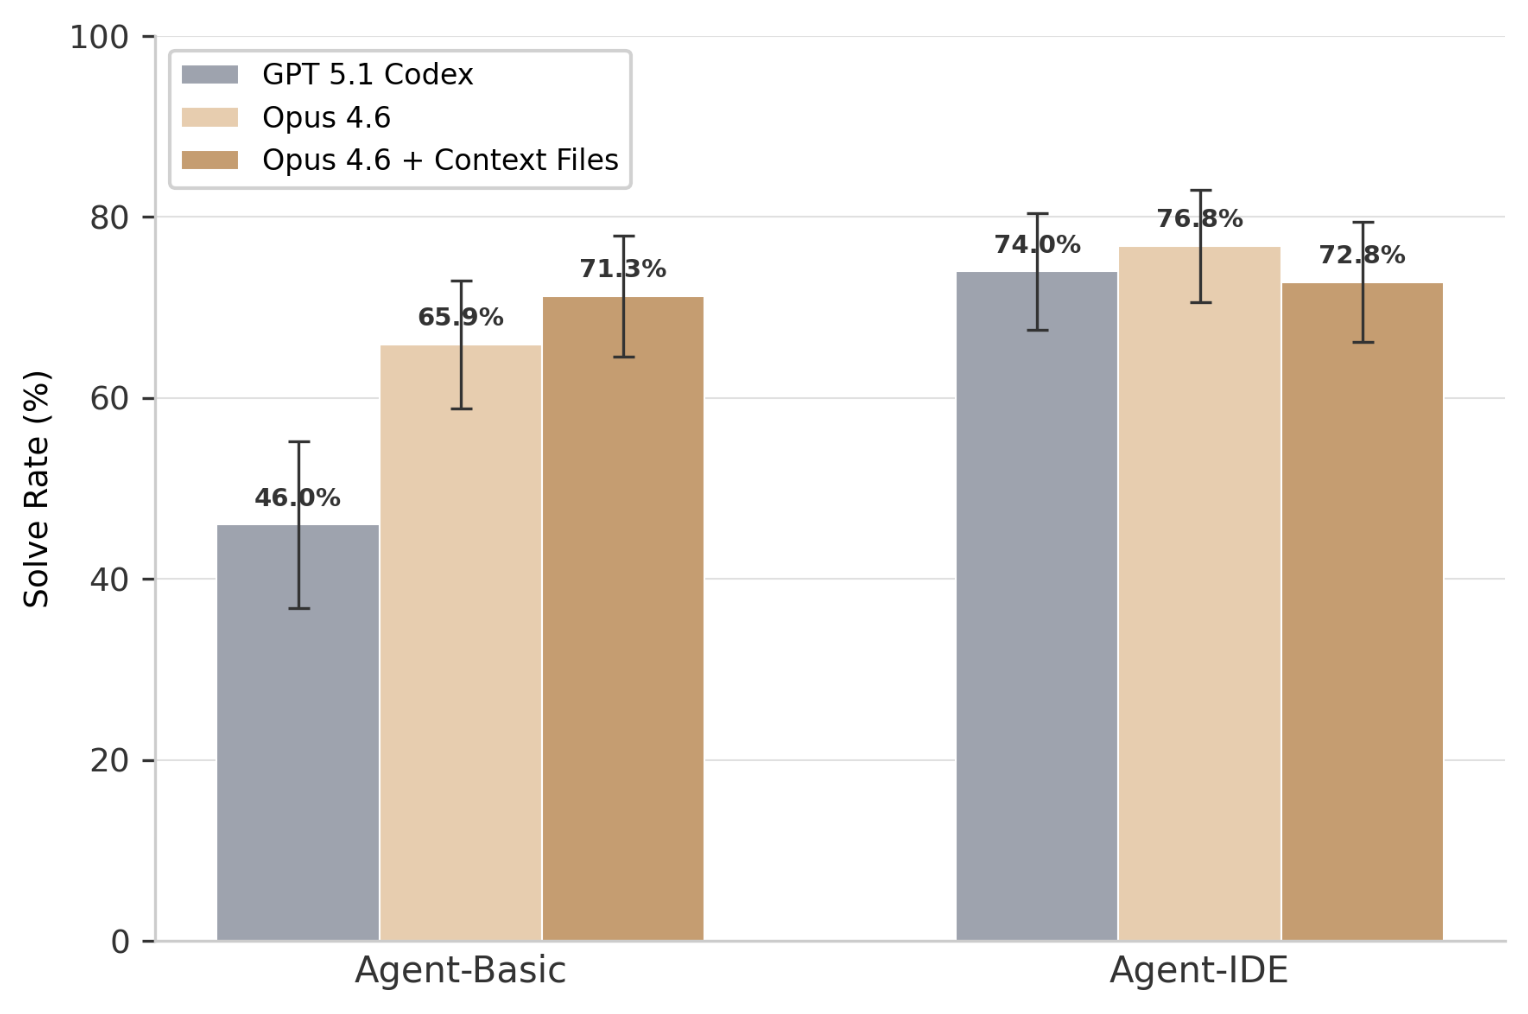
\includegraphics[width=0.9\columnwidth]{images/harness_evals.png}
\caption{\normalfont Harness evaluation comparison on \benchmark{}. Agent-Basic + Opus 4.6 significantly outperforms Agent-Basic + GPT 5.1 Codex. Despite search tool limitations on Agent-Basic, Opus 4.6 is able to navigate the codebase better. GPT 5.1 Codex often exhausts maximum iterations at evaluation time on Agent-Basic due to prolonged search operations (see Table~\ref{tab:tool_usage}). Agent-IDE outperforms Agent-Basic across Codex and Opus models. Agent-IDE has better code navigation which leads to fewer searches and better solve rates, see Table~\ref{tab:tool_usage} for tool usage comparison.}
\label{fig:harness-eval}
\end{figure}

\begin{table}[t]
\centering
\caption{\normalfont Tool usage distribution (\%) across harness + model. The table shows the top 7 tools used across the harnesses. Some tools like Todo Write are only available on Agent-IDE. Agent-Basic makes significantly more search tool calls compared to Agent-IDE. Opus 4.6 makes fewer search calls than GPT 5.1 Codex on Agent-Basic, but still considerably more than either model on Agent-IDE. Agent-IDE demonstrates better codebase navigation and code validation leading to overall higher solve rates on Agent-IDE harness.}
\label{tab:tool_usage}
\resizebox{\columnwidth}{!}{%
\begin{tabular}{lcccc}
\toprule
 & \multicolumn{2}{c}{\textbf{GPT 5.1 Codex}} & \multicolumn{2}{c}{\textbf{Opus 4.6}} \\
\cmidrule(lr){2-3} \cmidrule(lr){4-5}
Tool & Agent-Basic & Agent-IDE & Agent-Basic & Agent-IDE \\
\midrule
Read File & 28.9 & 27.8 & 36.8 & 26.5 \\
Search Files & 48.5 & 11.6 & 31.4 & 13.4 \\
Shell & 8.6 & 5.8 & 17.0 & 6.1 \\
Todo Write & --- & 14.6 & --- & 13.7 \\
Edit & 11.5 & --- & 9.1 & --- \\
Str Replace Edit & --- & 8.7 & --- & 9.4 \\
Validate Changes & 1.5 & 5.8 & 4.0 & 6.3 \\
\bottomrule
\end{tabular}%
}
\end{table}


\subsection{Empirical Validation of Automated Curation}
\label{subsec:manual-verification}

To validate the accuracy of the LLM-powered classifiers used in our curation pipeline, we conducted a manual verification study with two annotators, the first two authors of this paper, each with over five years of software engineering experience. Initial inter-annotator agreement exceeded 80\% for both tasks; dubious cases were discussed to reach consensus.

\subsubsection{Task Classification Accuracy}
We sampled 30 tasks (15 testable, 15 non-testable) and had both annotators independently judge testability. Since the pipeline's decision is binary (testable vs.\ non-testable), we compute agreement on this dimension. Annotators also labeled the fine-grained task type to enable qualitative comparison with the classifier's reasoning.

The classifier achieved 96.67\% agreement with the human consensus on the binary testability decision (29/30 cases). The single disagreement involved a prompt where the classifier labeled the task as testable (\texttt{bug\_fix}), while annotators reached consensus on non-testable (\texttt{debug\_investigation}). The prompt reported a potential bug after a recent diff, but did not explicitly request a fix; the developer appeared to be investigating whether the behavior change was intentional. This subtle distinction between reporting a potential bug and requesting a fix was missed by the classifier.

\subsubsection{Test Relevance Accuracy}

We sampled 15 (diff, test) pairs and had both annotators independently judge whether the test was relevant to the code change. We established three criteria for relevance: (1) the test directly exercises the modified function or class, (2) the test exercises code that depends on the modified module as a helper or utility, or (3) the test resides in the same test file or module as the changed code. A test is considered \textit{not relevant} if there is no verified control flow path between the test and the modified code.

\begin{itemize}
    \item \textbf{False negatives (2 cases):} The classifier rejected tests that annotators deemed relevant. In one case, the classifier's decision was reasonable, the test appeared to be a generic smoke test unrelated to the specific code change. However, annotators noted the original diff author had included this test in their test plan. In another, the test resided in the same test suite and exercised related functionality of the changed module, but the classifier rejected it since it did not test the specific feature being modified.
    \item \textbf{False positive (1 case):} The classifier accepted a test based on module-level proximity, reasoning that the test ``likely exercises workflow runs and health checks.'' However, annotators determined there was no actual import chain between the test and the modified code; they resided in the same conceptual software component but were functionally unrelated.
\end{itemize}

These disagreements occur at the subjective boundary of what constitutes ``relevance'' particularly for regression tests that reside in the same module but do not directly exercise the changed functionality. The classifier tends toward conservative decisions, which is preferable for benchmark quality as it reduces false positive test selections.

\begin{insight}
Both LLM-powered classifiers achieve high agreement with human annotators (96.67\% for task classification, 80\% for test relevance). Disagreements occur at subjective boundaries, investigative vs.\ action-oriented prompts for task classification, and module-level vs.\ function-level relevance for test selection. The classifiers' conservative tendencies align with benchmark quality goals.
\end{insight}

%% ============================================================================
\section{Related Work}
\label{sec:related}

\subsection{Benchmarks for Code Generation and Software Engineering Agents}

The evaluation of AI-assisted code generation has progressed through two distinct phases. The first generation of benchmarks, including HumanEval~\cite{chenEvaluatingLargeLanguage2021}, MBPP~\cite{austinProgramSynthesisLarge2021}, APPS~\cite{hendrycksMeasuringCodingChallenge2021}, and CodeContests~\cite{liCompetitionlevelCodeGeneration2022}, evaluates the ability of large language models to synthesize standalone functions from natural language specifications. These benchmarks measure \emph{functional correctness}, whether generated code passes a suite of unit tests, but abstract away the complexity inherent in professional software development: navigating large codebases, resolving cross-file dependencies, and integrating changes into existing systems.

The second generation addresses these limitations by situating evaluation within realistic repository contexts. SWE-bench~\cite{jimenezSWEbenchCanLanguage2024} pioneered this approach by constructing tasks from real GitHub issues paired with their corresponding pull request solutions, using the repository's test suite as an oracle. This benchmark, along with its human-validated subset SWE-bench Verified~\cite{IntroducingSWEbenchVerified} and training-oriented variant SWE-Gym~\cite{panTrainingSoftwareEngineering2025}, has become the primary evaluation standard for software engineering agents. Subsequent work has extended this paradigm to additional programming languages: SWE-Sharp-Bench~\cite{mhatreSWESharpBenchReproducibleBenchmark2025} targets C\#, SWE-PolyBench~\cite{rashidSWEPolyBenchMultilanguageBenchmark2025} covers Java, JavaScript, and TypeScript, and Multi-SWE-bench~\cite{zanMultiSWEbenchMultilingualBenchmark2025} spans seven languages. CrossCodeEval~\cite{dingCrossCodeEvalDiverseMultilingual2023} further evaluates cross-file code completion capabilities.

\benchmark{} shares the repository-level evaluation paradigm with SWE-bench but differs in one aspect: the source of natural language task specifications. Existing benchmarks derive their prompts from GitHub issue descriptions, text written to communicate with other developers, not to instruct an AI system. In contrast, \benchmark{} captures the \emph{verbatim prompts} that developers typed into an AI coding assistant. This distinction matters because issue descriptions often assume shared context, reference external resources, or describe symptoms rather than desired behavior, whereas prompts to AI assistants tend to be more self-contained and action-oriented.

\subsection{Developer Interactions with AI Coding Assistants}

Understanding how developers actually interact with AI coding tools helps construct representative benchmarks. Several empirical studies have investigated these interaction patterns. Barke et al.~\cite{barkeGroundedCopilotHow2023} conducted an observational study of 20 programmers using GitHub Copilot and identified two primary interaction modes: \emph{acceleration mode}, where developers have a clear goal and use the AI to implement it faster, and \emph{exploration mode}, where developers are uncertain and use the AI to discover possible approaches. Vaithilingam et al.~\cite{vaithilingamExpectationVsExperience2022} found that while Copilot did not consistently improve task completion time, developers valued it for providing useful starting points and reducing the need to search documentation. Studies of developer trust~\cite{brownIdentifyingFactorsThat2024} have shown that acceptance of AI suggestions depends on factors including suggestion quality, the developer's expertise in the relevant language, and the development context (e.g., production code versus tests).

Other work has examined how developers communicate with conversational AI assistants. Xiao et al.~\cite{xiaoDevGPTStudyingDeveloperChatGPT2024} curated a dataset of developer conversations with ChatGPT shared on GitHub, enabling analysis of real-world usage patterns. Khojah et al.~\cite{khojahHumantoHumanHumantoBotConversations2024} compared conversations between developers and those between developers and AI assistants, finding fundamental differences in structure and content. Mozannar et al.~\cite{mozannarReadingLinesModeling2024} developed a model of user behavior when interacting with code completion systems, quantifying the time costs of different interaction patterns.

These studies reveal a gap that \benchmark{} addresses: while we understand increasingly more about how developers interact with AI tools, existing benchmarks do not capture these authentic interactions. By sourcing tasks from actual usage of an AI coding assistant, \benchmark{} provides evaluation data that reflects real developer intent and communication patterns, complementing insights from observational studies with a benchmark grounded in authentic use.

\subsection{Benchmark Quality and Reinforcement Learning for Code}

The reliability of benchmark-driven evaluation depends on data quality. Two challenges are particularly relevant: test flakiness and data contamination. Flaky tests, tests that produce non-deterministic outcomes without changes to the code under test, can introduce noise into evaluation metrics~\cite{parrySurveyFlakyTests2021}. \benchmark{} mitigates this through multi-run stability checks that exclude tasks where test outcomes vary across executions. Data contamination occurs when benchmark data appears in model training corpora, leading to inflated performance estimates. LiveCodeBench~\cite{jainLiveCodeBenchHolisticContamination2024} addresses this by continuously collecting new problems from programming competitions, ensuring temporal separation from training data. \benchmark{} adopts a similar \emph{rolling benchmark} design, periodically refreshing the task set with recent samples that post-date model training cutoffs.

Beyond evaluation, execution-based signals from test suites can guide model improvement. Research in automated program repair (APR) has demonstrated that large language models, when combined with test feedback, can substantially outperform traditional template-based repair techniques~\cite{xiaAutomatedProgramRepair2023}. Conversational approaches such as ChatRepair~\cite{xiaAutomatedProgramRepair2024} further improve repair effectiveness by iteratively refining patches based on test failure information. This principle extends to model training: reinforcement learning methods can use test outcomes as reward signals. CodeRL~\cite{leCodeRLMasteringCode2022} introduced an actor-critic framework where a critic network predicts functional correctness to provide training signal, while RLEF~\cite{gehringRLEFGroundingCode2025} demonstrated that models trained to leverage execution feedback require an order of magnitude fewer samples to achieve comparable performance. \benchmark{} is designed to support such training paradigms, with its test classification scheme (fail-to-pass, pass-to-pass, extra tests) enabling fine-grained reward signal construction.

%% ============================================================================
\section{Threats to Validity}
\label{sec:limitations}

\paragraph{Construct Validity.}
The multi-stage filtering pipeline reduces the initial corpus to a few hundred benchmark instances, trading data volume for quality. This reduction constrains applicability for reward-signal-based post-training via reinforcement learning (RL), which typically requires corpora of tens of thousands of labeled trajectories to achieve stable policy improvement. Furthermore, by construction, \benchmark{} is restricted to single-turn interactions, in which the developer issues one prompt and the agent produces a complete code change without further dialogue. While this design simplifies evaluation, it systematically excludes tasks that require iterative refinement, multi-step debugging, or collaborative problem decomposition. These are common interaction patterns that occur in professional software development and likely represent a qualitatively harder class of agentic tasks.

\paragraph{Internal Validity.}
The evaluation harness exposes a set of tools to the agent under evaluation, some of which may inadvertently disclose privileged information. In particular, a tool that retrieves the current local diff could expose the \emph{backout diff}, the inverse patch that would revert the committed change, effectively leaking the ground-truth solution and compromising evaluation integrity. Additionally, approximately 65\% of the retained high-quality diffs exhibit 100\% AI provenance, meaning every character in the committed change originated from AI-generated suggestions that the developer accepted without modification. Consequently, these instances function as \emph{self-consistency} checks rather than independent evaluations: the benchmark measures whether the agent can reproduce a solution it (or a model of the same family) previously generated, rather than solving a novel task. This conflation of evaluation and training distribution warrants careful interpretation of reported solve rates.

\paragraph{External Validity.}
State-of-the-art models currently achieve a solve rate of approximately 70\%, indicating that a fraction of benchmark instances may be insufficiently challenging. This ceiling effect limits the benchmark's discriminative power for distinguishing among frontier models and raises the question of whether the selected tasks are representative of the full complexity of real-world software engineering. Further, the benchmark may not reflect the programming language distribution, coding conventions, or task complexity found in all development environments.

\paragraph{Reliability.}
To mitigate threats to reliability, \benchmark{} employs multi-run stability checks that exclude tasks where test outcomes vary across executions, reducing the impact of flaky tests on evaluation metrics. Each model is evaluated three times to quantify variance in reported solve rates. Nevertheless, the rolling benchmark design, in which stale samples are periodically replaced with fresh ones, means that two evaluations conducted at different points in time are not directly comparable, and longitudinal performance trends should be interpreted with caution.

\subsection{Planned Improvements}

Future work will address these threats along several dimensions. To improve pipeline throughput, we plan to parallelize base-commit test execution and introduce caching of backout-diff results, reducing end-to-end benchmark construction time. To improve environment faithfulness, we will incorporate recorded workspace snapshots to restore the exact set of local, uncommitted changes visible to the developer at authoring time. To address the ceiling effect and expand task diversity, we will broaden the data funnel to include diffs from multi-turn conversations and alternative AI coding assistants, and will specifically target scenarios requiring deeper reasoning, cross-file coordination, or domain-specific knowledge.

%% ============================================================================
\section{Conclusion}
\label{sec:conclusion}

This paper presented a methodology for curating production-derived benchmarks for AI coding agents, illustrated through \benchmark{}.
Our data collection and curation practices, including LLM-based task classification, test relevance validation, and multi-run stability checks, address challenges in constructing reliable evaluation signals from monorepo environments.
By preserving verbatim prompts and supporting seven programming languages, the resulting benchmark reflects real-world usage patterns that differ from existing benchmarks derived from GitHub issues.

Our systematic analysis of four foundation models revealed solve rates ranging from \SolveRateLowest{}\% to \SolveRateHighest{}\%, with higher-performing models exhibiting greater use of work validation tools, suggesting that iterative verification improves agent effectiveness. Harness evaluation results show how strong toolsets can improve task performance.

The methodology and lessons learned are designed to be replicable: organizations can follow this approach to construct analogous benchmarks from their own production data.
